\section{Exercise: Comparing Relaxed-Clock Models \& Estimating Time-Calibrated Phylogenies}

\subsection{Introduction}

Central among the questions explored in biology are those that seek to understand the timing and rates of evolutionary processes. Accurate estimates of species divergence times are vital to understanding historical biogeography, estimating diversification rates, and identifying the causes of variation in rates of molecular evolution. 

This tutorial will provide a general overview of divergence time estimation using fossil calibration and relaxed-clock model comparison in a Bayesian framework. The exercise will guide you through the steps necessary for estimating phylogenetic relationships and dating species divergences using the program \href{https://github.com/revbayes/revbayes}{\RevBayes}. 

%\begin{figure}[h!]
%\centering
%\fbox{\includegraphics[width=3in]{figures/yule_gm.eps}}
%\caption{\small The graphical model representation of the pure-birth (Yule) process conditioned on the orgin time.}
%\label{yuleGMfig}
%\end{figure}
%

\bigskip
\subsection{Getting Started}\label{gettingStarted}


The various exercises in this tutorial take you through the steps required to perform phylogenetic analyses of the example datasets. 
In addition, we have provided the output files for every exercise so you can verify your results. (Note that since the MCMC runs you perform will start from different random seeds, the output files resulting from your analyses \textit{will not} be identical to the ones we provide you.)

\begin{framed}
Download the starting tree file: \href{http://bit.ly/1tFOXXX}{http://bit.ly/1tFOXXX}

Download the alignment file: \href{http://bit.ly/1xs6pEd}{http://bit.ly/1xs6pEd}
\end{framed}

In this exercise, we will compare among different relaxed clock models and estimate a posterior distribution of calibrated time trees.
The dataset we will use is an alignment of 10 caniform sequences, comprising 8 bears, 1 spotted seal, and 1 gray wolf. 
Additionally, we will use occurrence times from three caniform fossils to calibrate our analysis to absolute time (Table \ref{bearFossilTable}).

\begin{table}[tbh!]
\centering
\caption{Fossil species used for calibrating divergence times in the caniform tree.}\label{bearFossilTable}
\begin{tabular}{@{\extracolsep{\fill}}l  c c c r}
\hline
\multicolumn{1}{@{}l}{\textbf{Fossil species}}  & &\multicolumn{1}{c}{\textbf{Age range (My)}}  & &\multicolumn{1}{c}{\textbf{Citation}} \\ 
\hline
\textit{Hesperocyon gregarius} & \hspace{2mm} & 37.2--40 & \hspace{2mm} & \cite{wang1994,wang1999}\\
\textit{Parictis montanus} & & 33.9--37.2 &  & \cite{clark1972,krause2008}\\
\textit{Kretzoiarctos beatrix} & & 11.2--11.8 &  & \cite{abella2011,abella12}\\
\hline
\end{tabular}
\end{table}


The alignment in file \cl{data/bears\_irbp.nex} contains interphotoreceptor retinoid-binding protein (irbp) sequences for each extant species.



\bigskip
\subsection{Creating Rev Files}

This tutorial sets up three different relaxed clock models and a calibrated birth-death model. 
Because of the complexity of the various models, this exercise is best performed by specifying the models and samplers in different \Rev~files.
At the beginning of each section, you will be given a suggested name for each component file; these names correspond to the provided \Rev~scripts that reproduce these commands.

\textbf{\textit{Directory Structure}}

This tutorial assumes that you have a very specific directory structure when running \RevBayes. 
First, you may want to put the \RevBayes~binary in your path if you're using a Unix-based operating system.
Alternatively, you can place the binary in a directory from which you will execute \RevBayes, e.g., the tutorial directory. 
The tutorial directory can be any directory on your file system, but you may want to create a new one so that you avoid conflicts with other \RevBayes~tutorials.

\begin{framed}
Create a directory for this tutorial called {\textcolor{red}{\cl{RB\_RelaxedClock\_Tutorial}}} (or any name you like), and navigate to that directory. This is the tutorial directory mentioned above.
\end{framed}

For this exercise, the \Rev~code provided assumes that within the tutorial directory exists  subdirectories. 
These directories must have the same names given here, unless you wish to also change the \Rev~code to conform to your specific directory names.

The first subdirectory will contain the data files (downloaded in Section \ref{gettingStarted}).
\begin{framed}
Create a directory called {\textcolor{red}{\cl{data}}} in your tutorial directory. 

Save the tree and alignment files downloaded above (Section \ref{gettingStarted}) in the \cl{data} directory.
\end{framed}

The second subdirectory will contain the \Rev~files you write to execute the exercises in this tutorial. 
\begin{framed}
Create a directory called {\textcolor{red}{\cl{RevBayes\_scripts}}} in your tutorial directory. 
\end{framed}
This tutorial will guide you through creating all of the files necessary to execute the analyses without typing the \Rev~language syntax directly in the \RevBayes~console. 
Since the scripts must point to model and analysis files in a modular way, it is important to be aware of you directory structure and if you choose to do something different, make sure that the file paths given throughout the tutorial are correct.

Finally, we'll need a directory for all of the files written by our analyses. For some operations, \RevBayes~can create this directory on the fly for you. 
However, it may be safer just to add it now.
\begin{framed}
Create a directory called {\textcolor{red}{\cl{output}}} in your tutorial directory.
\end{framed}

The only files you need for this exercise are now in the \cl{data} directory. Otherwise, you will create all of the \Rev~files specifying the models and analyses. 
All of the \Rev~files you write for this tutorial are available on the \href{https://github.com/revbayes/revbayes}{\RevBayes~GitHub repository} at this URL: \href{http://bit.ly/1zj5u9n}{http://bit.ly/1zj5u9n}.
You can refer to these examples to verify your own work.

\bigskip
\subsection{Calibrating the Birth-Death Model}\label{brMods} 

Fortunately, the fossil record for caniforms (and other carnivores) is quite good. 
We must formulate a birth-death model that accounts for the fossil occurrence times in Table \ref{bearFossilTable}. 
This part of the exercise will involve specifying a birth-death model with clamped stochastic nodes representing the observation times of two fossils descended from internal nodes in our tree: (1) \textit{Parictis montanus}, the oldest fossil in the family Ursidae, a stem fossil bear, and (2) \textit{Kretzoiarctos beatrix}, the fossil Ailuropodinae, a crown fossil bear.
Additionally, we will use the canid fossil, \textit{Hesperocyon gregarius}, to offset the age of the root of the tree. 

In \RevBayes, calibrated internal nodes are treated differently than in many other programs for estimating species divergence times (e.g., BEAST).
This is because the graphical model structure used in \RevBayes~does not allow a stochastic node to be assigned more than one prior distribution. 
By contrast, the common approach to applying calibration densities as used in other dating softwares leads to incoherence in the calibration prior \citep[for detailed explainations of this see][]{warnock12,heled12,heath2013fossilized}. 
More explicitly, common calibration approaches assume that the age of a calibrated node is modeled by the tree-wide diversification process (e.g., birth-death model) \textit{and} a parametric density parameterized by the occurrence time of a fossil (or other external prior information).
This can induce a calibration prior density that is not consistent with the birth-death process or the parametric prior distribution. 
Thus, approaches that condition the birth-death process on the calibrated nodes are more statistically coherent \citep{yang06}.

In \RevBayes, calibration densities are applied in a different way, treating fossil observation times like data. 
The graphical model in Figure \ref{m_BDCal:fig} illustrates how calibrated nodes are specified in the directed acyclic graph (DAG).
Here, the age of the calibration node (i.e., the internal node specified as the MRCA of the fossil and a set of living species) is a deterministic node---e.g., denoted $o_1$ for fossil $\mathcal{F}_1$---and acts as an offset on the stochastic node representing the age of the fossil specimen.
The fossil age, $\mathcal{F}_i$, is specified as a stochastic node and clamped to its \textit{observed} age in the fossil record. 
The node $\mathcal{F}_i$ is modeled using a distribution that describes the waiting time from the speciation event to the appearance of the observed fossil. 
Thus, if the MCMC samples any state of $\Psi$ for which the age of $\mathcal{F}_i$ has a probability of 0, then that state will always be rejected, effectively calibrating the birth-death process without applying multiple prior densities to any calibrated node (Fig.~\ref{m_BDCal:fig}).

The root age is treated differently, however. 
Here, we condition the birth-death process on the speciation time of the root, thus this variable is not part of the time-tree parameter. 
The root age can thus be given any parametric distribution over positive real numbers (Fig.~\ref{m_BDCal:fig}).

\begin{figure}[h!]
\centering
\fbox{\includegraphics[width=6in]{RB_RelaxedClock_Tutorial/figures/calib_BDR_gm.eps}}
\caption{\small The graphical model representation of the node-calibrated birth-death process in \RevBayes.}
\label{m_BDCal:fig}
\end{figure}

\textbf{\textit{Create the Rev File}}

{\begin{framed}
Open your text editor and create the birth-death model file called {\textcolor{red}{\cl{m\_BDP\_bears.Rev}}} in the \cl{RevBayes\_scripts} directory.

Enter the \Rev~code provided in this section in the new model file.
\end{framed}}


\textbf{\textit{Read in the Starting Tree}}

When calibrating nodes in the birth-death process, it is very helpful to have a starting tree that is consistent with the topology constraints and calibration priors, otherwise, the probability of the model would be 0 and the MCMC cannot run.
For a starting tree we will use the tree estimated by \citet{dosReis2012}. 
{\tt \begin{snugshade*}
\begin{lstlisting}
T <- readTrees("data/bears_dosReis.tre")[1]
\end{lstlisting}
\end{snugshade*}}

From the tree we can initialize some useful variables.
{\tt \begin{snugshade*}
\begin{lstlisting}
n_taxa <- T.ntips()
names <- T.names()
\end{lstlisting}
\end{snugshade*}}

%And our move-index iterator.
%{\tt \begin{snugshade*}
%\begin{lstlisting}
%mi = 1
%\end{lstlisting}
%\end{snugshade*}}

\subsubsection{Birth-Death Parameters}

We will begin by setting up the model parameters and proposal mechanisms of the birth-death model. 
Note that we have not initialized the workspace iterator \cl{mi} yet. 
Because of this, if you typed these lines in the \RevBayes~console, you would get an error. 
Since this code is intended to be in a sourced \Rev~file, we are assuming that you would initialize \cl{mi} before calling \cl{source("RevBayes\_scripts/m\_BDP\_Tree\_bears.Rev")}.

We will use the parameterization of the birth-death process specifying the diversification and turnover.
For a more detailed tutorial on the simple birth-death model, please refer to the tutorial in the \RevBayes~repository: \href{http://bit.ly/10UKeuq}{http://bit.ly/10UKeuq}.

\textbf{\textit{Diversification}}

Diversification ($d$) is the speciation rate ($\lambda$) minus the extinction rate ($\mu$): $d = \lambda - \mu$.
{\tt \begin{snugshade*}
\begin{lstlisting}
diversification ~ dnExponential(10.0) 
moves[mi++] = mvScale(diversification,lambda=1.0,tune=true,weight=3.0)
\end{lstlisting}
\end{snugshade*}}

\textbf{\textit{Turnover}}

Turnover is: $r = \mu / \lambda$.
{\tt \begin{snugshade*}
\begin{lstlisting}
turnover ~ dnBeta(2.0, 2.0) 
moves[mi++] = mvSlide(turnover,delta=1.0,tune=true,weight=3.0)
\end{lstlisting}
\end{snugshade*}}

\textbf{\textit{Deterministic Nodes for Birth and Death Rates}}

The birth rate and death rate are deterministic functions of the diversification and turnover.
First, create a deterministic node for $1 - r$, which is the denominator for each formula.

{\tt \begin{snugshade*}
\begin{lstlisting}
denom := abs(1.0 - turnover) 
\end{lstlisting}
\end{snugshade*}}

Now, the rates will both be positive real numbers that are variable transformations of the stochastic variables.
{\tt \begin{snugshade*}
\begin{lstlisting}
birth_rate := diversification / (denom)
death_rate := (turnover * diversification) / (denom)
\end{lstlisting}
\end{snugshade*}}

\textbf{\textit{Sampling Probability}}

Fix the probability of sampling to a known value. Since there are approximately 147 described caniform species, we will create a constant node for this parameter.
{\tt \begin{snugshade*}
\begin{lstlisting}
rho <- 0.068
\end{lstlisting}
\end{snugshade*}}

\subsubsection{Prior on the Root Node}

The fossil \textit{Hesperocyon gregarius} is a fossil descendant of the most-recent common ancestor of all caniformes and has an occurrence time of $\sim$38 Mya.
Thus, we can assume that the probability of the root age being younger than 38 Mya is equal to 0, using this value to offset a prior distribution on the root-age.

First specify the occurrence-time of the fossil.
{\tt \begin{snugshade*}
\begin{lstlisting}
tHesperocyon <- 38.0
\end{lstlisting}
\end{snugshade*}}

We will assume a lognormal prior on the root age that is offset by the observed age of \textit{Hesperocyon gregarius}. 
We can use the previous analysis by \citet{dosReis2012} to parameterize the lognormal prior on the root time. 
The age for the MRCA of the caniformes reported in their study was $\sim$49 Mya. 
Therefore, we can specify the mean of our lognormal distribution to equal $49 - 38 = 11$ Mya.
Given the expected value of the lognormal (\cl{mean\_ra}) and a standard deviation (\cl{stdv\_ra}), we can also compute the location parameter of the lognormal (\cl{mu\_ra}).
{\tt \begin{snugshade*}
\begin{lstlisting}
mean_ra <- 11.0
stdv_ra <- 0.25
mu_ra <- ln(mean_ra) - ((stdv_ra*stdv_ra) * 0.5)
\end{lstlisting}
\end{snugshade*}}

With these parameters we can instantiate the root age stochastic node with the offset value.
{\tt \begin{snugshade*}
\begin{lstlisting}
root_time ~ dnLognormal(mu_ra, stdv_ra, offset=tHesperocyon)
\end{lstlisting}
\end{snugshade*}}


\subsubsection{Topology Constraints \& Time Tree}

To create the tree with calibrated nodes, we must constrain the topology such that the calibrated nodes always have the same descendants.

The two non-root nodes we are calibrating in this tree is the MRCA of all living bears:
{\tt \begin{snugshade*}
\begin{lstlisting}
clade_Ursidae <- clade("Ailuropoda_melanoleuca","Tremarctos_ornatus","Helarctos_malayanus", "Ursus_americanus","Ursus_thibetanus","Ursus_arctos","Ursus_maritimus","Melursus_ursinus")
\end{lstlisting}
\end{snugshade*}}

And the MRCA of all bears and pinnipeds. 
{\tt \begin{snugshade*}
\begin{lstlisting}
clade_UrsPinn <- clade("Ailuropoda_melanoleuca","Tremarctos_ornatus","Helarctos_malayanus", "Ursus_americanus","Ursus_thibetanus","Ursus_arctos","Ursus_maritimus","Melursus_ursinus", "Phoca_largha")
\end{lstlisting}
\end{snugshade*}}

Once we have a set of constraints, we can use the vector function \cl{v()} to bind them in a constant vector.
{\tt \begin{snugshade*}
\begin{lstlisting}
constraints <- v(clade_Ursidae, clade_UrsPinn)
\end{lstlisting}
\end{snugshade*}}

Now we have all of the elements needed to specify the time-tree parameter.
{\tt \begin{snugshade*}
\begin{lstlisting}
timetree ~ dnBDP(lambda=birth_rate, mu=death_rate, rho=rho, rootAge=root_time, samplingStrategy="uniform", condition="nTaxa", nTaxa=n_taxa, names=names,constraints=constraints)
\end{lstlisting}
\end{snugshade*}}


\subsubsection{Calibrating Constrained Nodes}

In order that our tree is consistent with the calibration ages, we must first set the value of the time-tree node to our starting tree.
{\tt \begin{snugshade*}
\begin{lstlisting}
timetree.setValue(T)
\end{lstlisting}
\end{snugshade*}}

To begin specifying the calibration density on the MRCA of all ursids, we must first create the deterministic node representing the age of the MRCA.
The way in which these densities work requires the offset to be negative. 
Therefore we are creating two deterministic variables, one positive for monitoring, and one negative for the off-set.
We use the \cl{tmrca()} function to create these nodes which require that you provide a clade constraint.
{\tt \begin{snugshade*}
\begin{lstlisting}
tmrca_Ursidae := tmrca(timetree,clade_Ursidae)
n_TMRCA_Ursidae := -(tmrca_Ursidae)
\end{lstlisting}
\end{snugshade*}}

Now, we must specify our fossil occurrence time.
This is the age for the fossil panda, \textit{Kretzoiarctos beatrix}.
Note that we also make this value negative.
{\tt \begin{snugshade*}
\begin{lstlisting}
tKretzoiarctos <- -11.2
\end{lstlisting}
\end{snugshade*}}

Create the stochastic node for the age of the crown ursid fossil, using a lognormal distribution.
{\tt \begin{snugshade*}
\begin{lstlisting}
M <- 10
sdv <- 0.25
mu <- ln(M) - ((sdv * sdv) * 0.5)
crown_Ursid_fossil ~ dnLnorm(mu, sdv, offset=n_TMRCA_Ursidae)
\end{lstlisting}
\end{snugshade*}}

Now clamp the fossil age stochastic node with the observation time of \textit{Kretzoiarctos beatrix}
{\tt \begin{snugshade*}
\begin{lstlisting}
crown_Ursid_fossil.clamp(tKretzoiarctos)
\end{lstlisting}
\end{snugshade*}}

Next we will create the variable for the age of the MRCA of all bears and pinnipeds.
{\tt \begin{snugshade*}
\begin{lstlisting}
tmrca_UrsidaePinn := tmrca(timetree,clade_UrsPinn)
n_TMRCA_UrsidaePinn := -(tmrca_UrsidaePinn)
\end{lstlisting}
\end{snugshade*}}

Set the observed time for the stem fossil bear.
{\tt \begin{snugshade*}
\begin{lstlisting}
tParictis <- -33.9
\end{lstlisting}
\end{snugshade*}}

Create the stochastic node using the exponential prior and clamp it with the observation time of the fossil.
{\tt \begin{snugshade*}
\begin{lstlisting}
stem_Ursid_fossil ~ dnExponential(lambda=0.0333, offset=n_TMRCA_UrsidaePinn)
stem_Ursid_fossil.clamp(tParictis)
\end{lstlisting}
\end{snugshade*}}

\subsubsection{Proposals on the Time Tree (Node Ages Only)}

Next, create the vector of moves. These tree moves act on node ages:
{\tt \begin{snugshade*}
\begin{lstlisting}
moves[mi++] = mvNodeTimeSlideUniform(timetree, weight=30.0)
moves[mi++] = mvSlide(root_time, delta=2.0, tune=true, weight=10.0)
moves[mi++] = mvScale(root_time, lambda=2.0, tune=true, weight=10.0)
moves[mi++] = mvTreeScale(tree=timetree, rootAge=root_time, delta=1.0, tune=true, weight=3.0)
\end{lstlisting}
\end{snugshade*}}

%And these change the tree topology. If we wish to keep the topology constant, then we can leave these moves out. Note that for some relaxed clock models (autocorrelated rates, DPP, random-local clock) tree topology moves often induce very long mixing times.
%{\tt \begin{snugshade*}
%\begin{lstlisting}
%moves[mi++] = mvNNI(timetree, weight=8.0)
%moves[mi++] = mvNarrow(timetree, weight=8.0)
%moves[mi++] = mvFNPR(timetree, weight=8.0)
%\end{lstlisting}
%\end{snugshade*}}
%

Now save and close the file called {\textcolor{red}{\cl{m\_BDP\_bears.Rev}}}. This file, with all the model specifications will be loaded by other \Rev~files. 

\bigskip
\subsection{Specifying Branch-Rate Models}\label{brMods} 

The next sections will walk you through setting up the files specifying different relaxed clock models. 
Each section will require you to create a separate \Rev~file for each relaxed clock model, as well as for each marginal-likelihood analysis.

\bigskip
\subsubsection{The Global Molecular Clock Model}\label{globalClockSec}

The global molecular clock assumes that the rate of substitution is constant over the tree and over time.
When estimating trees on an absolute time-scale, it is often necessary to parameterize relaxed clock models with two rates, a base rate which effectively scales the tree and a clock rate. 
Then, the absolute rate applied to the tree is a deterministic node (Fig.~\ref{m_GMC:fig}).

\begin{figure}[h!]
\centering
\fbox{\includegraphics[width=3in]{RB_RelaxedClock_Tutorial/figures/gmc_gm.eps}}
\caption{\small The graphical model representation of the global molecular clock model used in this exercise.}
\label{m_GMC:fig}
\end{figure}

\textbf{\textit{Create the Rev File}}

{\begin{framed}
Open your text editor and create the global molecular clock model file called {\textcolor{red}{\cl{m\_GMC\_bears.Rev}}} in the \cl{RevBayes\_scripts} directory.

Enter the \Rev~code provided in this section in the new model file. Keep in mind that we are creating modular model files that can be sourced by different analysis files. Thus, the \Rev~code below will still depend on variable initialized in different files.
\end{framed}}




\textbf{\textit{The Clock-Rate}}

We specify the absolute clock rate by first creating a node for the base rate.
This value is set to be drawn from a lognormal prior.
{\tt \begin{snugshade*}
\begin{lstlisting}
br_M <- 5.4E-3
br_s <- 0.05
br_mu <- ln(br_M) - ((br_s * br_s) * 0.5)
base_rate ~ dnLnorm(br_mu, br_s)
moves[mi++] = mvScale(base_rate,lambda=0.25,tune=true,weight=5.0)
\end{lstlisting}
\end{snugshade*}}

The clock-rate parameter is a stochastic node from a gamma distribution.
{\tt \begin{snugshade*}
\begin{lstlisting}
clock_rate ~ dnGamma(2.0,4.0)
moves[mi++] = mvScale(clock_rate,lambda=0.5,tune=true,weight=5.0)
\end{lstlisting}
\end{snugshade*}}

The absolute clock rate is the value on which the phylogenetic CTMC model depends. This is a deterministic node and equal to the product of the base rate and clock rate.
{\tt \begin{snugshade*}
\begin{lstlisting}
abs_clock_rt := clock_rate * base_rate
\end{lstlisting}
\end{snugshade*}}

\textbf{\textit{The Sequence Model and Phylogenetic CTMC}}

Specify the parameters of the GTR model and the moves to operate on them.
{\tt \begin{snugshade*}
\begin{lstlisting}
sf ~ dnDirichlet(v(1,1,1,1))
er ~ dnDirichlet(v(1,1,1,1,1,1))
Q := fnGTR(er,sf)
moves[mi++] = mvSimplexElementScale(er, alpha=10.0, tune=true, weight=3.0)
moves[mi++] = mvSimplexElementScale(sf, alpha=10.0, tune=true, weight=3.0)
\end{lstlisting}
\end{snugshade*}}

And instantiate the phyoCTMC.
{\tt \begin{snugshade*}
\begin{lstlisting}
phySeq ~ dnPhyloCTMC(tree=timetree, Q=Q, branchRates=abs_clock_rt, nSites=n_sites, type="DNA")
phySeq.clamp(D)
\end{lstlisting}
\end{snugshade*}}

This is all we will include in the global molecular clock model file. 

{\begin{framed}
Save and close the file called {\textcolor{red}{\cl{m\_GMC\_bears.Rev}}} in the \cl{RevBayes\_scripts} directory.
\end{framed}}



%Specify the work-space model object.
%{\tt \begin{snugshade*}
%\begin{lstlisting}
%mymodel = model(er)
%\end{lstlisting}
%\end{snugshade*}}
%
%\exs{The global-molecular clock model is specified in the file called \href{https://github.com/revbayes/revbayes/raw/development/tutorials/RB_TimeTree_Tutorials/RB_TimeTree_Exercise/RB_timetree_files/RevBayes_scripts/m_GMC_bears.Rev}{\cl{m\_GMC\_bears.Rev }}.}

\textbf{\textit{Estimate the Marginal Likelihood}}

Now we can use the model files we created and estimate the marginal likelihood under the global molecular clock model (and all other model settings). 
You can enter the following commands directly in the \RevBayes~console, or you can create another \Rev~script. 

{\begin{framed}
Open your text editor and create the marginal-likelihood analysis file under the global molecular clock model. Call the file: {\textcolor{red}{\cl{mlnl\_GMC\_bears.Rev}}} and save it in the \cl{RevBayes\_scripts} directory.
\end{framed}}


\textit{Load Sequence Alignment} --- Read in the sequences and initialize important variables.
{\tt \begin{snugshade*}
\begin{lstlisting}
D <- readDiscreteCharacterData(file="data/bears_irbp.nex")
n_sites <- D.nchar(1)
mi = 1
\end{lstlisting}
\end{snugshade*}}

\textit{The Calibrated Time-Tree Model} --- Load the calibrated tree model from file using the \cl{source()} function. Note that this file does not have moves that operate on the tree topology, which is helpful when you plan to estimate the marginal likelihoods and compare different relaxed clock models.
{\tt \begin{snugshade*}
\begin{lstlisting}
source("RevBayes_scripts/m_BDP_bears.Rev")
\end{lstlisting}
\end{snugshade*}}

\textit{Load the GMC Model File} --- Source the file containing all of the parameters of the global molecular clock model. This file is called {\textcolor{red}{\cl{m\_GMC\_bears.Rev}}}.

{\tt \begin{snugshade*}
\begin{lstlisting}
source("RevBayes_scripts/m_GMC_bears.Rev")
\end{lstlisting}
\end{snugshade*}}

We can now create our workspace model variable with our fully specified model DAG. 
We will do this with the \cl{model()} function and provide a single node in the graph (\cl{er}).
{\tt \begin{snugshade*}
\begin{lstlisting}
mymodel = model(er)
\end{lstlisting}
\end{snugshade*}}

\textit{Run the Power-Posterior Sampler and Compute the Marginal Likelihoods} --- With a fully specified model, we can set up the \cl{powerPosterior()} analysis to create a file of `powers' and likelihoods from which we can estimate the marginal likelihood using stepping-stone or path sampling. 
This method computes a vector of powers from a beta distribution, then executes an MCMC run for each power step while raising the likelihood to that power. In this implementation, the vector of powers starts with 1, sampling the likelihood close to the posterior and incrementally sampling closer and closer to the prior as the power decreases. 

First, we create the variable containing the power posterior. This requires us to provide a model and vector of moves, as well as an output file name. The \cl{cats} argument sets the number of power steps.
Once we have specified the options for our sampler, we can then start the run after a burn-in/tuning period.

{\tt \begin{snugshade*}
\begin{lstlisting}
pow_p = powerPosterior(mymodel, moves, "output/GMC_bears_powp.out", cats=50) 
pow_p.burnin(generations=5000,tuningInterval=200)
pow_p.run(generations=1000)  
\end{lstlisting}
\end{snugshade*}}

Compute the marginal likelihood using two different methods, stepping-stone sampling and path sampling. 
{\tt \begin{snugshade*}
\begin{lstlisting}
ss = steppingStoneSampler(file="output/GMC_bears_powp.out", powerColumnName="power", likelihoodColumnName="likelihood")
ss.marginal() 

### use path sampling to calculate marginal likelihoods
ps = pathSampler(file="output/GMC_bears_powp.out", powerColumnName="power", likelihoodColumnName="likelihood")
ps.marginal() 
\end{lstlisting}
\end{snugshade*}}

If you have entered all of this directly in the \RevBayes~console, you will see the marginal likelihoods under each method printed to screen. 
Otherwise, if you have created the separate \Rev~file 
{\textcolor{red}{\cl{m\_GMC\_bears.Rev}}} in the \cl{RevBayes\_scripts} directory, you now have to directly source this file in \RevBayes (after saving the up-to-date content). 

{\tt \begin{snugshade*}
\begin{lstlisting}
source("RevBayes_scripts/mlnl_GMC_bears.Rev")
\end{lstlisting}
\end{snugshade*}}

{\begin{framed}
Once you have completed this analysis, record the marginal likelihoods under the global molecular clock model in Table \ref{ssTable}.
\end{framed}}

\bigskip
\subsubsection{The Uncorrelated Lognormal Rates Model}\label{UCLNModelSec}

The uncorrelated lognormal (UCLN) model relaxes the assumption of a single-rate molecular clock. 
Under this model, the rate associated with each branch in the tree is a stochastic node.
Each branch-rate variable is drawn from the same lognormal distribution (Fig.~\ref{m_UCLN:fig}).

Given that we might not have prior information on the parameters of the lognormal distribution, we can assign hyper priors to these variables. 
Generally, it is more straightforward to construct a hyperprior on the expectation (i.e., the mean) of a lognormal density rather than the location parameter $\mu$. 
Here, we will assume that the mean branch rate is exponentially distributed and as is the stochastic node representing the standard deviation.
With these two parameters, we can get the location parameter of the lognormal by:
$$\mu = \log(M) - \frac{\sigma^2}{2}.$$
Thus, $\mu$ is a deterministic node, which is a function of $M$ and $\sigma$.

In Figure \ref{m_UCLN:fig}, we can represent the vector of $N$ branch rates using the plate notation. Additionally, each branch rate is rescaled by the base rate. 
\begin{figure}[h!]
\centering
\fbox{\includegraphics[width=3in]{RB_RelaxedClock_Tutorial/figures/ucln_gm.eps}}
\caption{\small The graphical model representation of the UCLN model used in this exercise.}
\label{m_UCLN:fig}
\end{figure}


%
%\textbf{\textit{Load the Sequence Data and Birth-Death Model}}
%
%{\tt \begin{snugshade*}
%\begin{lstlisting}
%D <- readDiscreteCharacterData(file="data/bears_irbp.nex")
%n_sites <- D.nchar(1)
%mi = 1
%\end{lstlisting}
%\end{snugshade*}}
%
%{\tt \begin{snugshade*}
%\begin{lstlisting}
%source("RevBayes_scripts/m_BDP_bears.Rev")
%\end{lstlisting}
%\end{snugshade*}}

\textbf{\textit{Create the Rev File}}

{\begin{framed}
Open your text editor and create the uncorrelated-lognormal relaxed-clock model file called {\textcolor{red}{\cl{m\_UCLN\_bears.Rev}}} in the \cl{RevBayes\_scripts} directory.

Enter the \Rev~code provided in this section in the new model file. Keep in mind that we are creating modular model files that can be sourced by different analysis files. Thus, the \Rev~code below will still depend on variable initialized in different files.
\end{framed}}


\textbf{\textit{The Base Clock Rate}}

As in the strict clock model above, we create a lognormally distributed stochastic node, representing the base rate.
{\tt \begin{snugshade*}
\begin{lstlisting}
br_M <- 5.4E-3
br_s <- 0.05
br_mu <- ln(br_M) - ((br_s * br_s) * 0.5)
base_rate ~ dnLnorm(br_mu, br_s)
moves[mi++] = mvScale(base_rate,lambda=0.25,tune=true,weight=5.0)
\end{lstlisting}
\end{snugshade*}}

\textbf{\textit{Independent Branch Rates}}

Before we can set up the variable of the branch-rate model, we must know how many branches exist in the tree.
{\tt \begin{snugshade*}
\begin{lstlisting}
n_branches <- 2 * n_taxa - 2
\end{lstlisting}
\end{snugshade*}}

We will start with the mean of the lognormal distribution, $M$ in Figure \ref{m_UCLN:fig}.
{\tt \begin{snugshade*}
\begin{lstlisting}
ucln_mean ~ dnExponential(2.0)
\end{lstlisting}
\end{snugshade*}}

And the exponentially distributed node representing the standard deviation.
We will also create a deterministic node, which is the variance, $\sigma^2$.
{\tt \begin{snugshade*}
\begin{lstlisting}
ucln_sigma ~ dnExponential(3.0)
ucln_var := ucln_sigma * ucln_sigma
\end{lstlisting}
\end{snugshade*}}

Now we can declare the function that gives us the $\mu$ parameter of the lognormal distribution on branch rates.
{\tt \begin{snugshade*}
\begin{lstlisting}
ucln_mu := ln(ucln_mean) - (ucln_var * 0.5)
\end{lstlisting}
\end{snugshade*}}

The only stochastic nodes we need to operate on for this part of the model are the lognormal mean ($M$ or \cl{ucln\_mean}) and the standard deviation ($\sigma$ or \cl{ucln\_sigma}).
{\tt \begin{snugshade*}
\begin{lstlisting}
moves[mi++] = mvScale(ucln_mean, lambda=1.0, tune=true, weight=4.0)
moves[mi++] = mvScale(ucln_sigma, lambda=0.5, tune=true, weight=4.0)
\end{lstlisting}
\end{snugshade*}}

With our nodes representing the $\mu$ and $\sigma$ of the lognormal distribution, we can create the vector of stochastic nodes for each of the branch rates using a \cl{for} loop. 
Within this loop, we also add the move for each branch-rate stochastic node to our moves vector.
{\tt \begin{snugshade*}
\begin{lstlisting}
for(i in 1:n_branches){
   branch_rates[i] ~ dnLnorm(ucln_mu, ucln_sigma)
   moves[mi++] = mvScale(branch_rates[i], lambda=1, tune=true, weight=2.)
}
\end{lstlisting}
\end{snugshade*}}

Because we are dealing with semi-identifiable parameters, it often helps to apply a range of moves to the variables representing the branch rates and branch times. This will help to improve the mixing of our MCMC.
Here we will add 2 additional types of moves that act on vectors.
{\tt \begin{snugshade*}
\begin{lstlisting}
moves[mi++] = mvVectorScale(branch_rates,lambda=1.0,tune=true,weight=2.0) 
moves[mi++] = mvVectorSingleElementScale(branch_rates,lambda=30.0,tune=true,weight=1.0) 
\end{lstlisting}
\end{snugshade*}}

We can combine the base rate and branch rates in a vector of deterministic nodes.
{\tt \begin{snugshade*}
\begin{lstlisting}
branch_subrates := branch_rates * base_rate
\end{lstlisting}
\end{snugshade*}}

The mean of the branch rates is a convenient deterministic node to monitor, particularly in the screen output when conducting MCMC.
{\tt \begin{snugshade*}
\begin{lstlisting}
mean_rt := mean(branch_rates) 
\end{lstlisting}
\end{snugshade*}}

\textbf{\textit{The Sequence Model and Phylogenetic CTMC}}

Now, specify the stationary frequencies and exchangeability rates of the GTR matrix.
{\tt \begin{snugshade*}
\begin{lstlisting}
sf ~ dnDirichlet(v(1,1,1,1))
er ~ dnDirichlet(v(1,1,1,1,1,1))
Q := fnGTR(er,sf)
moves[mi++] = mvSimplexElementScale(er, alpha=10.0, tune=true, weight=3.0)
moves[mi++] = mvSimplexElementScale(sf, alpha=10.0, tune=true, weight=3.0)
\end{lstlisting}
\end{snugshade*}}

Now, we can put the whole model together in the phylogenetic CTMC and clamp that node with our sequence data.
{\tt \begin{snugshade*}
\begin{lstlisting}
phySeq ~ dnPhyloCTMC(tree=timetree, Q=Q, branchRates=branch_subrates, nSites=n_sites, type="DNA")
attach the observed sequence data
phySeq.clamp(D)
\end{lstlisting}
\end{snugshade*}}

{\begin{framed}
Save and close the file called {\textcolor{red}{\cl{m\_UCLN\_bears.Rev}}} in the \cl{RevBayes\_scripts} directory.
\end{framed}}



\textbf{\textit{Estimate the Marginal Likelihood}}

Just as we did for the strict clock model, we can execute a power-posterior analysis to compute the marginal likelihood under the UCLN model. 

{\begin{framed}
Open your text editor and create the marginal-likelihood analysis file under the global molecular clock model. Call the file: {\textcolor{red}{\cl{mlnl\_UCLN\_bears.Rev}}} and save it in the \cl{RevBayes\_scripts} directory.
\end{framed}}

Refer to the section describing this process for the GMC model above.
Write your own \Rev~language script to estimate the marginal likelihood under the UCLN model. 
Be sure to change the file names in all of the relevant places (e.g., your output file for the \cl{powerPosterior()} function should be \colorbox{shadecolor}{\cl{UCLN\_bears\_powp.out}} and be sure to \cl{source()} the correct model file \colorbox{shadecolor}{\cl{source("RevBayes\_scripts/m\_UCLN\_bears.Rev")}}).

{\begin{framed}
Once you have completed this analysis, record the marginal likelihoods under the UCLN model in Table \ref{ssTable}.
\end{framed}}

\bigskip
\subsubsection{The Autocorrelated Lognormal Rates Model}\label{ACLNModelSec}

A model assuming that the rate at each node is lognormally distributed with a mean centered on its parent rate and a variance proportional to the time-duration since the parent node is an autocorrelated model \citep[ACLN;][]{thorne98,kishino01,thorne02}. 
This corresponds to a geometric Brownian motion model.
The ACLN model relies on the topology and branch-durations of the time-tree and is thus more complex to represent graphically.
Thus, we use the convenience of the tree plate to show the conditional dependence structure among node rates and ages in Figure \ref{m_ACLN:fig}.

\begin{figure}[h!]
\centering
\fbox{\includegraphics[width=6in]{RB_RelaxedClock_Tutorial/figures/acln_gm.eps}}
\caption{\small The graphical model representation of the ACLN model used in this exercise.}
\label{m_ACLN:fig}
\end{figure}

In this model, for any node (internal or tip) that is not the root, the rate at that node $r_i$ is drawn from a lognormal distribution with an expected value equal to the rate of the parent node $r_{\tilde{p}(i)}$ and a variance that is the product of the time difference $t_i$ and the variance parameter $\nu$. 
Note that the graphical model represented in Figure \ref{m_ACLN:fig} is simplified to to make it easier to understand, thus some deterministic nodes are obfuscated.  
Importantly, it is worth recognizing that the ACLN model describes the rate values at the \textit{nodes} of the tree and not the branches. 
Because of this, additional deterministic nodes are used to compute the rate along branch $i$, $b_i$, which is the average of the two nodes subtending that branch: $b_i = (r_i + r_{\tilde{p}(i)}) / 2$.

\textbf{\textit{Create the Rev File}}

{\begin{framed}
Open your text editor and create the autocorrelated-lognormal relaxed-clock model file called {\textcolor{red}{\cl{m\_ACLN\_bears.Rev}}} in the \cl{RevBayes\_scripts} directory.

Enter the \Rev~code provided in this section in the new model file. Keep in mind that we are creating modular model files that can be sourced by different analysis files. Thus, the \Rev~code below will still depend on variable initialized in different files.
\end{framed}}



\textbf{\textit{The Base Clock Rate}}

As in the strict clock and UCLN models above, we create a lognormally distributed stochastic node, representing the base rate.
{\tt \begin{snugshade*}
\begin{lstlisting}
br_M <- 5.4E-3
br_s <- 0.05
br_mu <- ln(br_M) - ((br_s * br_s) * 0.5)
base_rate ~ dnLnorm(br_mu, br_s)
moves[mi++] = mvScale(base_rate,lambda=0.25,tune=true,weight=5.0)
\end{lstlisting}
\end{snugshade*}}


\textbf{\textit{Autocorrelated Node Rates}}

Begin by declaring the parameters of the ACLN model. The first is the parameter \cl{nu} which determines the degree of autocorrelation among node rates. If \cl{nu} is very large, then the variance of the lognormal distribution on node rates is also very large, resulting in low autocorrelation. 
Conversely, if \cl{nu} is very small, then closely related nodes will have very similar rates.
And if \cl{nu = 0} the model collapses to a strict clock, where all nodes have the same substitution rate.
For this dataset we will assign an exponential prior to \cl{nu} with an expected value of 1.0 and use a scale-type move to propose changes.
{\tt \begin{snugshade*}
\begin{lstlisting}
nu ~ dnExponential(1.0)
moves[mi++] = mvScale(nu, lambda=0.5, tune=true, weight=4.0)
\end{lstlisting}
\end{snugshade*}}

The next parameter of the ACLN model is the rate value at the root of the tree. 
We will assume that this rate is drawn from a gamma distribution with an expected value of 0.5.
{\tt \begin{snugshade*}
\begin{lstlisting}
root_rate ~ dnGamma(2.0, 4.0)
moves[mi++] = mvScale(root_rate, lambda=0.5, tune=true, weight=4.0)
\end{lstlisting}
\end{snugshade*}}

Now we can declare our stochastic node containing the node rates. 
This is conditioned on the \cl{timetree} node we defined by our birth-death model, the variance parameter \cl{nu}, the \cl{root\_rate}, and the \cl{base\_rate}.
{\tt \begin{snugshade*}
\begin{lstlisting}
node_rates ~ dnACLN(timetree, nu, root_rate, base_rate)
\end{lstlisting}
\end{snugshade*}}

Because the ACLN model describes the distribution of rates at the nodes of the tree, we must compute the rate for each \textit{branch} as a vector of deterministic nodes. Where the rate for a given branch is the average of the rates a the nodes subtending that branch.
For this, we can use an explicit function written at the \Rev~language level that takes the tree and all other parameters of the ACLN model and looks up the relevant parameters for a given index. 
We can declare a vector of deterministic branch rates using a \cl{for} loop.
{\tt \begin{snugshade*}
\begin{lstlisting}
n_branches <- 2 * n_taxa - 2
for(i in 1:n_branches){
   branch_rates[i] := aveRateOnBranch(node_rates, timetree, root_rate, base_rate, index=i)
}
\end{lstlisting}
\end{snugshade*}}

The mean of the branch rates is a convenient deterministic node to monitor, particularly in the screen output when conducting MCMC.
{\tt \begin{snugshade*}
\begin{lstlisting}
mean_rt := mean(branch_rates) 
\end{lstlisting}
\end{snugshade*}}

Defining moves for a model like the ACLN is a bit tricky. Because of strong parameter interactions among all of the node rates and ages, the model doesn't mix well with standard moves. 
The autocorrelation may also make it difficult to efficiently sample the tree topology jointly under this model.
Thus, it is worth putting some thought into the MCMC proposals. 
In \RevBayes~there are two moves especially for the ACLN-distributed node rates.
The first, \cl{mvScaleSingleACLNRates}, selects a single non-root node at random and proposes a new value for the rate using a scale-type move. 
Because of the variance in rates across nodes, it is difficult to specify the move so that the tuning parameter is optimal for all nodes. 
Therefore, it may be necessary to declare multiple instances of this move with different tuning values that are not changed during burn-in.
Additionally, we can also add a move that is retuned so that the proposal size is optimal for the average node rate. 
{\tt \begin{snugshade*}
\begin{lstlisting}
moves[mi++] = mvScaleSingleACLNRates(node_rates, 4.0, false, n_branches)
moves[mi++] = mvScaleSingleACLNRates(node_rates, 2.0, false, n_branches)
moves[mi++] = mvScaleSingleACLNRates(node_rates, 3.0, true, 3* n_branches)
\end{lstlisting}
\end{snugshade*}}

The second move for ACLN node rates is a ``mixing step'' \citep{thorne98,kishino01,thorne02,rannala2003,yang06}.
This move rescales the node ages and proportionally changes the node rates so that the absolute branch lengths remain unchanged and the likelihood is unaffected.
This type of proposal can help your chain more efficiently sample parameter space without requiring costly recalculations of the model likelihood.
{\tt \begin{snugshade*}
\begin{lstlisting}
moves[mi++] = mvACLNMixingStep(timetree, node_rates, root_rate, 0.5, false, n_branches)
\end{lstlisting}
\end{snugshade*}}

\textbf{\textit{The Sequence Model and Phylogenetic CTMC}}

Now, specify the stationary frequencies and exchangeability rates of the GTR matrix.
{\tt \begin{snugshade*}
\begin{lstlisting}
sf ~ dnDirichlet(v(1,1,1,1))
er ~ dnDirichlet(v(1,1,1,1,1,1))
Q := fnGTR(er,sf)
moves[mi++] = mvSimplexElementScale(er, alpha=10.0, tune=true, weight=3.0)
moves[mi++] = mvSimplexElementScale(sf, alpha=10.0, tune=true, weight=3.0)
\end{lstlisting}
\end{snugshade*}}

Now, we can put the whole model together in the phylogenetic CTMC and clamp that node with our sequence data.
{\tt \begin{snugshade*}
\begin{lstlisting}
phySeq ~ dnPhyloCTMC(tree=timetree, Q=Q, branchRates=branch_subrates, nSites=n_sites, type="DNA")
attach the observed sequence data
phySeq.clamp(D)
\end{lstlisting}
\end{snugshade*}}

{\begin{framed}
Save and close the file called {\textcolor{red}{\cl{m\_ACLN\_bears.Rev}}} in the \cl{RevBayes\_scripts} directory.
\end{framed}}



\textbf{\textit{Estimate the Marginal Likelihood}}

Just as we did for the strict clock and UCLN models, we can execute a power-posterior analysis to compute the marginal likelihood under the ACLN model. 

{\begin{framed}
Open your text editor and create the marginal-likelihood analysis file under the global molecular clock model. Call the file: {\textcolor{red}{\cl{mlnl\_ACLN\_bears.Rev}}} and save it in the \cl{RevBayes\_scripts} directory.
\end{framed}}

Refer to the section describing this process for the GMC and UCLN models above.
Write your own \Rev~language script to estimate the marginal likelihood under the ACLN model. 
Be sure to change the file names in all of the relevant places.
Additionally, you may find that the power-posterior analysis runs too slow under this model, thus it may be advisable for you to decrease the number of cycles or tuning frequency in the burn-in period.

{\begin{framed}
Once you have completed this analysis, record the marginal likelihoods under the ACLN model in Table \ref{ssTable}.
\end{framed}}
% -2775.66

\FloatBarrier
\subsection{Compute Bayes Factors and Select Model}


Now that we have estimates of the marginal likelihood under each of our different models, we can evaluate their relative plausibility using Bayes factors.
Use Table \ref{ssTable} to summarize the marginal log-likelihoods estimated using the stepping-stone and path-sampling methods.
\begin{Form}
\begin{table}[h!]
\centering
\caption{\small Estimated marginal likelihoods for different across-branch substitution rate models$^*$.}
\begin{tabular}{l c c c c}
\hline
\multicolumn{1}{l}{\textbf{ }} &\multicolumn{1}{r}{\textbf{ }} & \multicolumn{3}{c}{\textbf{Marginal lnL estimates}} \\ 
\cline{3-5}
\multicolumn{1}{l}{\textbf{Clock Model}} & \multicolumn{1}{r}{\hspace{3mm}} & \multicolumn{1}{c}{\textit{Stepping-stone}} & \multicolumn{1}{r}{\hspace{3mm}} & \multicolumn{1}{c}{\textit{Path sampling}} \\ 
\hline
\ref{globalClockSec} Global molecular clock ($M_0$) & \hspace{15mm} & \TextField[name=m1,backgroundcolor={.85 .85 .85},color={1 0 0},height=4ex]{}  & \hspace{15mm} & \TextField[name=ml2,backgroundcolor={.85 .85 .85},color={0 0 1},height=4ex]{} \\
\hline
\ref{UCLNModelSec} Uncorrelated lognormal ($M_1$) & \hspace{3mm} &\TextField[name=ml3,backgroundcolor={.85 .85 .85},color={1 0 0},height=4ex]{}   & \hspace{3mm} & \TextField[name=ml4,backgroundcolor={.85 .85 .85},color={0 0 1},height=4ex]{} \\
\hline
\ref{ACLNModelSec} Autocorrelated lognormal ($M_2$) & \hspace{3mm} &\TextField[name=ml3,backgroundcolor={.85 .85 .85},color={1 0 0},height=4ex]{}   & \hspace{3mm} & \TextField[name=ml4,backgroundcolor={.85 .85 .85},color={0 0 1},height=4ex]{} \\
\hline
%\ref{mlnl_ACLN} Autocorrelated lognormal  ($M_2$) & \hspace{3mm} & \TextField[name=ml5,backgroundcolor={.85 .85 .85},color={1 0 0},height=4ex]{} & \hspace{3mm} & \TextField[name=ml6,backgroundcolor={.85 .85 .85},color={0 0 1},height=4ex]{} \\
{\footnotesize{$^*$you can edit this table}}\\
\end{tabular}
\label{ssTable}
\end{table}
\end{Form}

Phylogenetics software programs log-transform the likelihood to avoid \href{http://en.wikipedia.org/wiki/Arithmetic_underflow}{underflow}, because multiplying likelihoods results in numbers that are too small to be held in computer memory.
Thus, we must calculate the ln-Bayes factor (we will denote this value $\mathcal{K}$):
\begin{align}\label{LNbfFormula}
\mathcal{K}=\ln[BF(M_0,M_1)] = \ln[\mathbb{P}(\mathbf X \mid M_0)]-\ln[\mathbb{P}(\mathbf X \mid M_1)],
\end{align}
where $\ln[\mathbb{P}(\mathbf X \mid M_0)]$ is the \textit{marginal lnL} estimate for model $M_0$. 
The value resulting from equation \ref{LNbfFormula} can be converted to a raw Bayes factor by simply taking the exponent of $\cal{K}$
\begin{align}\label{LNbfFormula2}
BF(M_0,M_1) = e^{\cal{K}}.
\end{align}
Alternatively, you can interpret the strength of evidence in favor of $M_0$ using the $\cal{K}$ and skip equation \ref{LNbfFormula2}. 
In this case, we evaluate the $\cal{K}$ in favor of model $M_0$ against model $M_1$ so that:
\begin{center}
\begin{tabular}{l}
if $\mathcal{K} > 1$, then model $M_0$ wins\\
if $\mathcal{K} < -1$, then model $M_1$ wins.
\end{tabular}
\end{center}
Thus, values of $\mathcal{K}$ around 0 indicate ambiguous support. 


Using the values you entered in Table \ref{ssTable} and equation \ref{LNbfFormula},  calculate the ln-Bayes factors (using $\mathcal{K}$) for the different model comparisons. 
Enter your answers in Table \ref{bfTable} using the stepping-stone and the path-sampling estimates of the marginal log likelihoods. 

\begin{Form}
\begin{table}[h!]
\centering
\caption{\small Bayes factor calculation based on marginal likelihood estimates in Table \ref{ssTable}$^*$.}
\begin{tabular}{l c c c c}
\hline
\multicolumn{1}{l}{\textbf{ }} &\multicolumn{1}{r}{\textbf{ }} & \multicolumn{3}{c}{\textbf{ln-Bayes Factor} ($\mathcal{K}$)} \\ 
\cline{3-5}
\multicolumn{1}{l}{\textbf{Model comparison}} & \multicolumn{1}{r}{\hspace{3mm}} & \multicolumn{1}{c}{\textit{Stepping-stone}} & \multicolumn{1}{r}{\hspace{3mm}} & \multicolumn{1}{c}{\textit{Path sampling}} \\ 
\hline
$M_0,M_1$ & \hspace{15mm} & \TextField[name=ml7,backgroundcolor={.85 .85 .85},color={1 0 0},height=4ex]{}  & \hspace{15mm} & \TextField[name=ml8,backgroundcolor={.85 .85 .85},color={0 0 1},height=4ex]{} \\
$M_0,M_2$ & \hspace{15mm} & \TextField[name=ml7,backgroundcolor={.85 .85 .85},color={1 0 0},height=4ex]{}  & \hspace{15mm} & \TextField[name=ml8,backgroundcolor={.85 .85 .85},color={0 0 1},height=4ex]{} \\
$M_1,M_2$ & \hspace{15mm} & \TextField[name=ml7,backgroundcolor={.85 .85 .85},color={1 0 0},height=4ex]{}  & \hspace{15mm} & \TextField[name=ml8,backgroundcolor={.85 .85 .85},color={0 0 1},height=4ex]{} \\
\hline
Supported model? & \hspace{3mm} &  \TextField[name=ml13,backgroundcolor={1 .85 .85},color={1 0 0},height=4ex]{} & \hspace{3mm} & \TextField[name=ml14,backgroundcolor={.85 .85 1},color={0 0 1},height=4ex]{} \\
\hline
{\footnotesize{$^*$you can edit this table}}\\
\end{tabular}
\label{bfTable}
\end{table}
\end{Form}

\bigskip
\subsection{Estimate the Topology and Branch Times}

After computing the Bayes factors and determining the relative support of each model, you can choose your favorite model among the three tested in this tutorial. 
The next step, then, is to use MCMC to jointly estimate the tree topology and branch times. 

{\begin{framed}
Open your text editor and create the MCMC analysis file under the your favorite clock model. Call the file: {\textcolor{red}{\cl{mcmc\_TimeTree\_bears.Rev}}} and save it in the \cl{RevBayes\_scripts} directory.
\end{framed}}

This file will contain much of the same initial \Rev~code as the files you wrote for the marginal-likelihood analyses. 

{\tt \begin{snugshade*}
\begin{lstlisting}
### Load the sequence alignment
D <- readDiscreteCharacterData(file="data/bears_irbp.nex")

### get helpful variables from the data
n_sites <- D.nchar(1)

### initialize an iterator for the moves vector
mi = 1
\end{lstlisting}
\end{snugshade*}}

This is how you should begin your MCMC analysis file. The next step is to source the birth-death model. 
However, if you're interested in estimating the tree topology, then you must add proposals that will do this.
These moves can be added right after the birth-death model is sourced.
{\tt \begin{snugshade*}
\begin{lstlisting}
### set up the birth-death model from file
source("RevBayes_scripts/m_BDP_bears.Rev")

### and moves for the tree topology
moves[mi++] = mvNNI(timetree, weight=8.0)
moves[mi++] = mvNarrow(timetree, weight=8.0)
moves[mi++] = mvFNPR(timetree, weight=8.0)
\end{lstlisting}
\end{snugshade*}}

Next load the file containing your favorite model (where the wildcard \cl{*} indicates the name of the model you prefer: \cl{GMC}, \cl{UCLN}, or \cl{ACLN}).
{\tt \begin{snugshade*}
\begin{lstlisting}
### load the model from file 
source("RevBayes_scripts/m_*_bears.Rev")

### workspace model wrapper ###
mymodel = model(er)
\end{lstlisting}
\end{snugshade*}}

\textbf{\textit{MCMC Monitors}}

Before you instantiate the MCMC workspace object, you need to create a vector of ``monitors'' that are responsible for monitoring parameter values and saving those to file or printing them to the screen. 

First, create a monitor of all the model parameters except the \cl{timetree} using the model monitor: \cl{mnModel}.
This monitor takes \textit{all} of the named parameters in the model DAG and saves their value to a file. 
Thus, every variable that you gave a name in your model files will be written to your log file. 
This makes it very easy to get an analysis going, but can generate very large files with a lot of redundant output. 
{\tt \begin{snugshade*}
\begin{lstlisting}
monitors[1] = mnModel(filename="output/TimetTree_bears_mcmc.log", printgen=10)
\end{lstlisting}
\end{snugshade*}}

If the model monitor is too verbose for your needs, you should use the file monitor instead: \cl{mnFile}. For this monitor, you have to provide the names of all the parameters you're interested in after the file name and print interval. 
(Refer to the example files for how to set up the file monitor for model parameters.)

In fact, we use the file monitor for saving the sampled chronograms to file. 
It is important that you \textit{do not} save the sampled trees in the same file with other numerical parameters you would like to summarize. That is because tools for reading MCMC log files---like \href{http://tree.bio.ed.ac.uk/software/tracer/}{Tracer} \citep{rambaut09}---cannot load files with non-numerical states.
Therefore, you must save the sampled trees to a different file.
{\tt \begin{snugshade*}
\begin{lstlisting}
monitors[2] = mnFile(filename="output/TimeTree_bears_mcmc.trees", printgen=10, timetree)
\end{lstlisting}
\end{snugshade*}}


Finally, we will create a monitor in charge of writing information to the screen: \cl{mnScreen}.
We will report the root age and base rate to the screen. If there is anything else you'd like to see in your screen output (e.g., the mean rate of the UCLN or ACLN model), feel free to add them to the list of parameters give to this model.
{\tt \begin{snugshade*}
\begin{lstlisting}
monitors[3] = mnScreen(printgen=10, root_time, base_rate)
\end{lstlisting}
\end{snugshade*}}

\textbf{\textit{Setting-Up \& Executing the MCMC}}

Now everything is in place to create the MCMC object in the workspace.
This object allows you to perform a burn-in, execute a run of a given length, continue an analysis that might not have reached stationarity, and summarize the performance of the various proposals.
{\tt \begin{snugshade*}
\begin{lstlisting}
mymcmc = mcmc(mymodel, monitors, moves)
\end{lstlisting}
\end{snugshade*}}

With this object instantiated, specify a burn-in period that will sample parameter space while re-tuning the proposals (only for the moves with \cl{tune=true}). 
The monitors do not sample the states of the chain during burn-in.
{\tt \begin{snugshade*}
\begin{lstlisting}
mymcmc.burnin(generations=2000,tuningInterval=100)
\end{lstlisting}
\end{snugshade*}}

Once the burn-in is complete, we want the analysis to run the full MCMC. 
Specify the length of the chain. 
{\tt \begin{snugshade*}
\begin{lstlisting}
mymcmc.run(generations=5000)
\end{lstlisting}
\end{snugshade*}}

When the MCMC run has completed, it's often good to evaluate the acceptance rates of the various proposal mechanisms. 
The \cl{.operatorSummary()} member method of the MCMC object prints a table summarizing each of the parameter moves to the screen. 
{\tt \begin{snugshade*}
\begin{lstlisting}
mymcmc.operatorSummary()
\end{lstlisting}
\end{snugshade*}}

\textbf{\textit{Summarize the Sampled Time-Trees}}

During the MCMC, the sampled trees will be written to a file that we will summarize using the \cl{mapTree} function in \RevBayes.
This first requires that you add the code for reading in the tree-trace file and performing an analysis of those trees.
{\tt \begin{snugshade*}
\begin{lstlisting}
tt = readTreeTrace("output/TimeTree_bears_mcmc.trees", "clock")
tt.summarize()

### write MAP tree to file
mapTree(tt, "output/TimeTree_bears_mcmc_MAP.tre")
\end{lstlisting}
\end{snugshade*}}

{\begin{framed}
Save and close the file called {\textcolor{red}{\cl{mcmc\_TimeTree\_bears.Rev}}} in the \cl{RevBayes\_scripts} directory. 
Then, execute the MCMC analysis using: \colorbox{shadecolor}{\cl{source("RevBayes\_scripts/mcmc\_TimeTree\_bears.Rev")}}
\end{framed}}


\bigskip
\section*{Useful Links}

\begin{itemize}
\item RevBayes: \href{https://github.com/revbayes/revbayes}{https://github.com/revbayes/revbayes} \\ \vspace{-7mm}
\item Tree Thinkers: \href{http://treethinkers.org/}{http://treethinkers.org} \\ \vspace{-7mm}
\end{itemize}

Questions about this tutorial can be directed to: \\\vspace{-10mm}
\begin{itemize}
\item Tracy Heath (email: \href{mailto:tracyh@berkeley.edu}{tracyh@berkeley.edu}) \\\vspace{-8mm}
\item Tanja Stadler (email: \href{mailto:tanja.stadler@bsse.ethz.ch}{tanja.stadler@bsse.ethz.ch}) \\\vspace{-8mm} 
\item Sebastian H\"{o}hna (email: \href{mailto:sebastian.hoehna@gmail.com}{sebastian.hoehna@gmail.com})
\end{itemize}


\bibliographystyle{mbe}
\bibliography{bib_tex/master_refs}
